\chapter{Discussions \& Conclusions}
The implementation details of the tool have been explained in depth. Some of the design decisions which has been made during the development of the tool have also been briefly discussed.
This discussion chapter will dive more into the details of the development process, and elaborate more on what else was tried and tested to achieve the current result.

This chapter will elaborate on the important discussion topics being made throughout the development process of the tool, and explain how
some of the bigger design decisions were made.

The chapter will also discuss what similar tools exist and how the tool compares to these tools. Lastly, how the tool can be developed further to enhance user experience, and what features and changes could be made to the tool to either make it more useable
or solve more problems for the user. This will also serve as a discussion of the shortcomings of the tool.

All sections of this chapter will also have a small conclusive part to each of the aspects. This means that no separate conclusion chapter will follow this chapter.

\section{Reconnaissance}
The tool has been through one major revision before reaching the state that it is in now. This section
will explain the \emph{first version} of the tool, briefly how it was implemented, and why the revision was needed.
The first version served as a way to get familiar with visualization and D3.js. It was also a tool where different approaches were tested to see what works and what does not.

The general structure of the tool was very different. The first version tried to be more decoupled from VS Code than what the tool currently is.
The first version was a Java program which had an open server socket. From this server socket, a lot of endpoints were exposed which would serve the whole user interface as well as provide the Jolie system JSON data.
This approach requires that a port is open on the machine whenever the tool is running.

It was never tested with VS Code so it is not certain how VS Code would incorporate a tool like this. One idea is
that the tool must be running on the host machine, essentially as a server, and a client in VS Code would need to fetch the user interface from the specified endpoints.
The client in the VS Code extension would be a web view as it is at the moment.
Whenever an update to the Jolie code is made the client in the VS Code web view will have to fetch data from all endpoints again.

\subsection{The Program Inspector}
To get the JSON data from the Java service, an internal \texttt{ProgramInspector} was used to fetch the information about the Jolie services. This inspector exists within the Jolie parser but has limitations with how it gathers information about services.
It looks at a file and gathers all information meaning that if multiple services exist in one file, the ProgramInspector will not differentiate between components in one service and components in another service.
When the ProgramInspector has gathered all the AST nodes of a Jolie source file, the JSON objects are created directly. No internal representation of each component was created for this version of the tool.

Another problem with the first version is that no sense of top-level services is present. The tool simply parses all files in the root directory recursively. This creates a lot of bloating of the visualization and JSON data because unwanted services, interfaces, and types may be present in the user interface.
This resulted in all services, both top-level and embeddings being in one global list of services.
This is ultimately why the architecture file is introduced. So the user can specify exactly what services in what files should be parsed and visualized in the user interface. The other benefit of the architecture file is that the user of the tool can specify parameters for the visualization and prototyping of the services.

\subsection{User Interface}
In the first version of the tool, the user interface is vastly different. A lot of inspiration was taken from the documentation of Jolie.\footnote{An example of how services are displayed in the Jolie documentation - \url{https://docs.jolie-lang.org/v1.10.x/language-tools-and-standard-library/architectural-patterns/synchronous-vs-asynchronous/index.html}}
This shape of services is easy to implement because they all have a direction, all input ports are on one side and all output ports are on the opposite side.

\cref{figure:old_ui} shows a very early version of how the user interface displayed the service shapes. This is without any layout algorithm being applied to the service which is why all services are next to each other.
The red triangles on the left side of the service shapes represent the output ports and the yellow squares on the right side represent the input ports, and the height of the service is simply determined by how many ports it needs to fit.

The problem with this approach is that in some architectures, the visualization can be very hard to understand.
It gives the sense that there exists some sort of direction or flow between services which is not necessarily the case.
Embeddings are not represented intuitively. If a service is embedded by another service it is simply placed to the left of the embedder service and a dashed square is drawn around the two services indicating that an embedding is happening, but it 
is not clear to an inexperienced Jolie developer what is the embedder service and what is the embedded service.
This is why the current version of the tool has chosen a more \emph{traditional} approach to the service shapes. It does not imply a flow and it can be easier to visualize more complicated architectures.

The UI for the first version is grid-based where all services can be moved around and will snap to the grid.
The reason a grid is used is that the edges that represent the connection between ports are calculated using the \emph{A*} pathfinding algorithm\footnote{A* pathfinding algorithm - \url{https://en.wikipedia.org/wiki/A*_search_algorithm}}, so each point in the grid is essentially used as a point in a graph that the pathfinding algorithm can use.
This also means that invisible walls are created around the services and ports to ensure that paths do not go through other services or ports.
The current version of the tool has hexagons as service shapes, so to facilitate the possibility of having ports on all sides of the shape, the pathfinding from the output port to the input port must be handled differently.
One idea which was tried is connecting services instead of ports, and then drawing the port shapes at the edge of the service shape where the connection intersects the service shape.
A grid is not used in the current version of the tool because ELK is used to make the edges between ports.

\begin{figure}[t]
\center
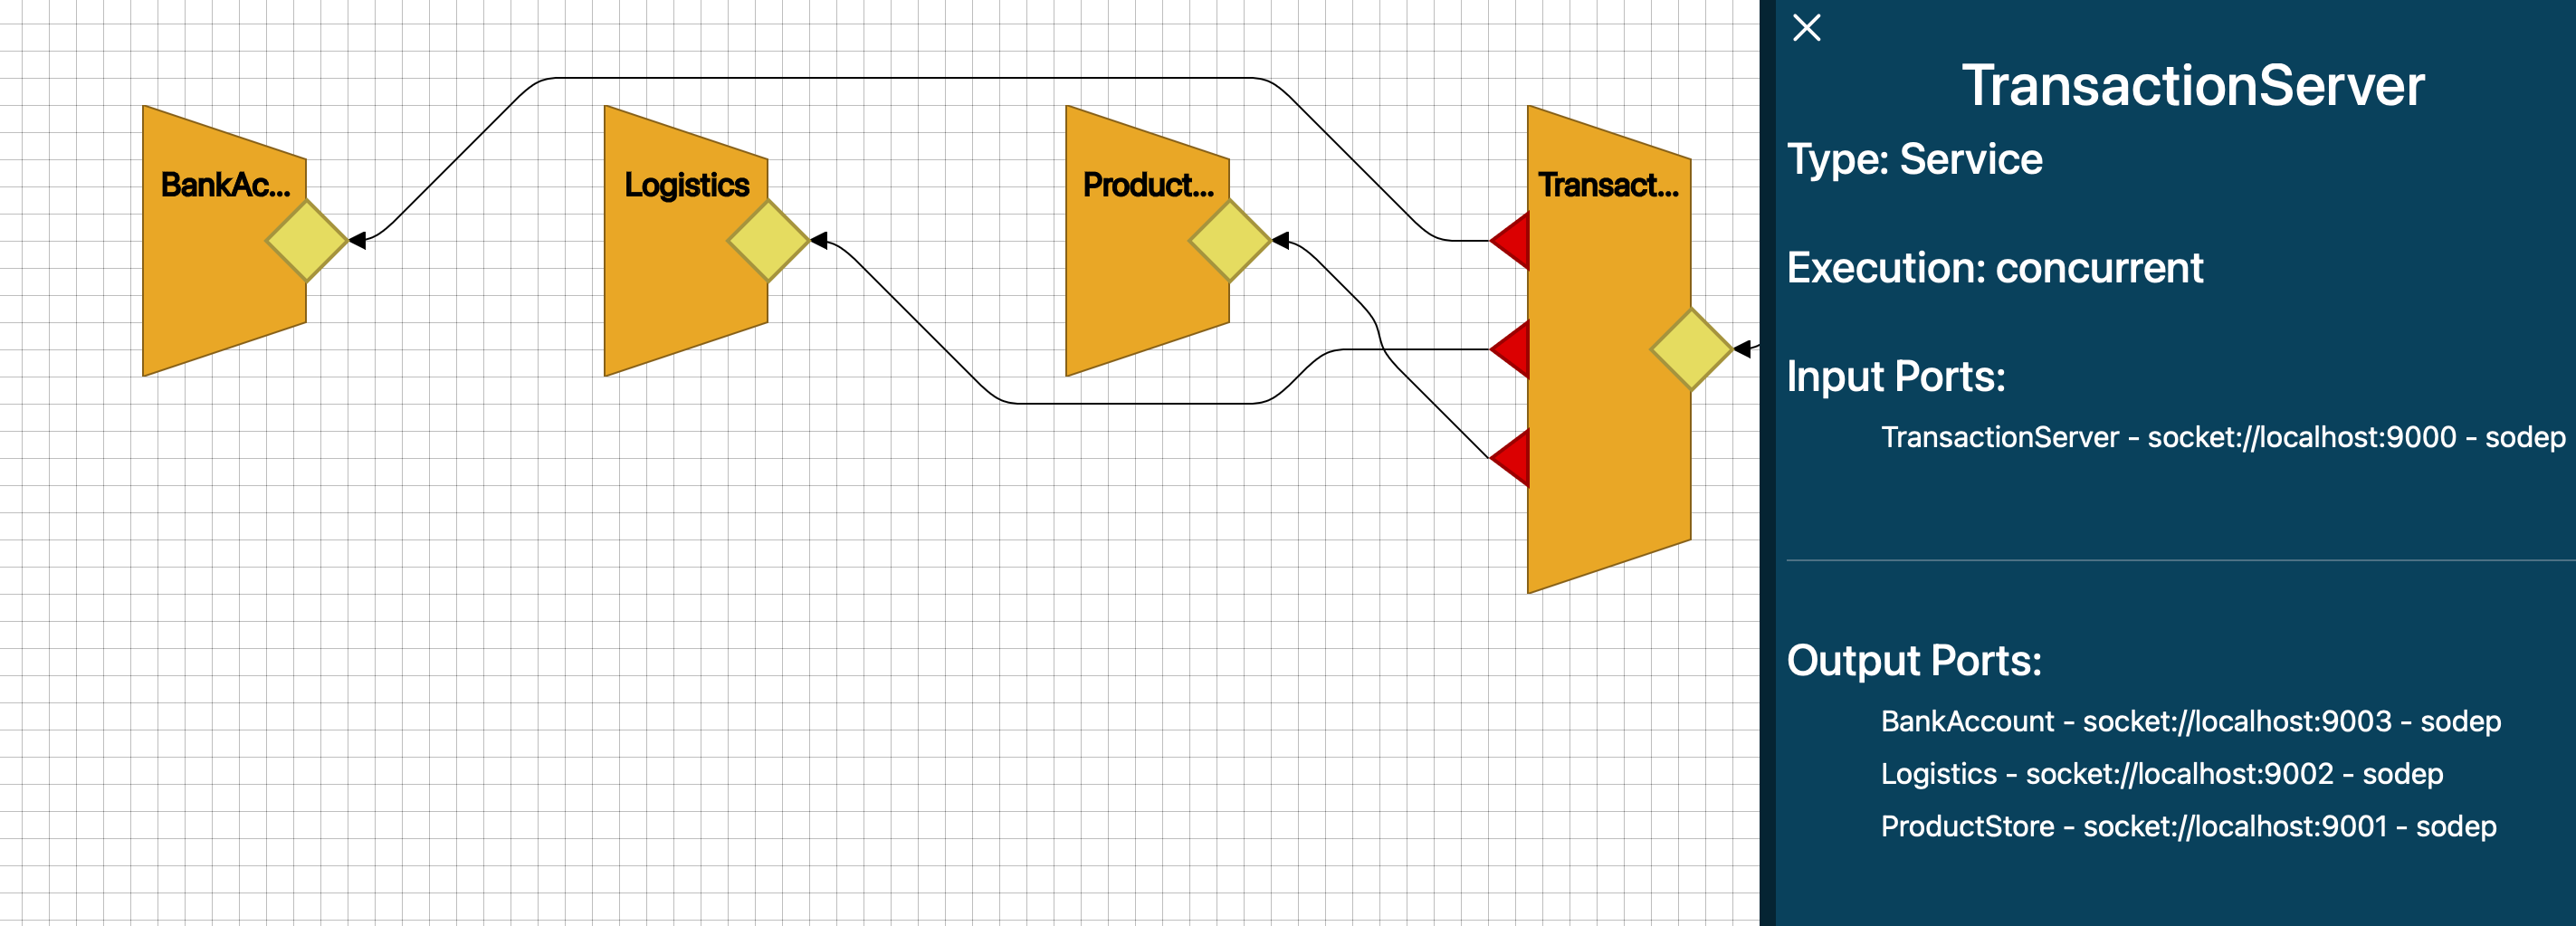
\includegraphics[width=0.8\textwidth]{figures/old_ui.png}
\caption{A very early version of how the first version of the tool displayed service shapes and the sidebar. No layout algorithm is used to place the services correctly on the grid in this version.}
\label{figure:old_ui}
\end{figure}

\subsection{Layout Algorithm}
The first version of the tool uses a simple custom layered layout algorithm. This is possible because the services have a direction.
The algorithm works by placing each service in a horizontal layer based on how many of each port it has. The starting number of layers is determined by the width of the screen and each layer has a set height limit so when services exceed the limit an adjacent layer is created.
Services with only one input port are placed in the left-most layer, and services with only one output layer are placed in the right-most layer.
The services in between will be ordered so the service with most \emph{connected} ports will be placed in the middle-most layer and services with an input port connected to an output port of the middle service will be placed to the left. Services having output ports connected to input ports of the middle service are placed to the right.

This algorithm is very simple. It worked on the handful of tested examples from the Jolie GitHub repository.\footnote{Jolie Examples on GitHub - \url{https://github.com/jolie/examples/tree/master}}
But when the system becomes more complex connection-wise, it can quickly break or incomprehensible. One advantage of using this algorithm is that the user can drag around the services if the initial layout is bad.

The algorithm does not necessarily break because of the hexagon shapes which were introduced after. The switch to ELK was made because connections can become complex, and having a highly customizable framework is much safer in terms of the systems the tool will potentially have to visualize.
ELK uses a variety of researched layout algorithms which are more robust than the simpler layout algorithm which was used before.

\subsection{UI Framework}
The introduction of a UI framework was made because of the component tree, lifecycle events, and reactivity. Before Svelte was used to create the user interface, it was created in pure TypeScript.
The UI in the first version has no lifecycle events, all JavaScript is loaded after the DOM is created.
The control flow of the user interface is that after the DOM has loaded all the Jolie system JSON data is loaded and preprocessed very similarly to the current version, but here, the custom layout algorithm is used.
Then all components are added to the DOM, under one parent container, using jQuery\footnote{jQuery - \url{https://jquery.com}} and rendered using D3.js. Lastly, the event listeners are added to the system components. The event listeners include the mouse listener for moving the service shapes around and opening the sidebar to display information about the components.
When the user interface is updated by the user, a re-rendering happens. Since all system DOM elements are added under one parent container element, that specific element is simply cleared and the rendering is invoked to populate it with the updated elements.

This approach of using pure TypeScript/JavaScript is not inherently wrong. After all, Svelte compiles down to optimized JavaScript.
There are general benefits and consequences of using a UI framework. Some of the important benefits are efficiency in handling reactivity, reusable components, and enhanced maintainability.
Efficient reactivity means no manual manipulation of the DOM is necessary. The code will update the state of the components which automatically updates the DOM.
Some of the consequences of using a UI framework are the learning curve, performance, and framework-specific limitations.
Some UI frameworks have a steep learning curve, especially for newer web developers, so having to learn and understand the framework can in some cases take more time than just implementing the functionality in JavaScript.
The performance is not necessarily a problem for Svelte since the overhead is minimal, but for larger UI frameworks like React and Angular, performance can become an issue since they ship a virtual DOM\footnote{React virtual DOM - \url{https://legacy.reactjs.org/docs/faq-internals.html}} which in VS Code can be a bottleneck.
For this specific tool, there are no apparent framework-specific limitations with Svelte, which is one of the reasons it was chosen.

\section{Control Flow} % subsection?
Having a simple control flow is key to preventing bugs, keeping the tool fast, and making the tool easier to extend and maintain.
Different flows were tested to see which gave the best results in terms of speed but also the experience from the perspective of the user.
The first version did not have many flows. The initialization was simple but this version of the tool did not have refactoring capabilities, so comparing it with the current solution is unnecessary.

The current flow has split up the different operations so they happen both in the user interface and the code simultaneously, without interfering with each other. Another approach which was tried is to have the user interface update from the newly refactored code. This means that when the UI sends a refactoring request to VS Code, the UI does not update, but waits for VS Code to send the updated JSON back to the UI.
This approach is simpler than the one used currently but with a significant performance decrease compared to the current solution.

The current solution is chosen because it is faster. The updates happen in parallel which is faster from the perspective of the user because the UI shows the changes immediately instead of waiting for the VS Code extension to update. The control flow might not be as simple as the first proposed solution, but it is still easy to understand.

\section{Data Representation}
Different representations of the Jolie system JSON were tested. There are some tradeoffs to consider when structuring the JSON which can affect size and computation in the user interface.
The interface list in the JSON does not have to be a global array. Interfaces are only used by ports which reside in the services, structurally, and at the moment the interfaces in a port simply contain the name and file path pair of the interfaces used. This could be switched out with the whole interface object.
This would, however, result in at least twice the size of all interfaces, because each time an interface is used the whole interface JSON object is created. Input and output ports share interfaces which means that for every connection between ports, an interface is duplicated.

The global list of types has a similar problem but can be avoided a bit easier. Types can be created under the interfaces which use them, which would remove the need for a global list, but again if the interfaces are created under ports, each type will be duplicated in the JSON. 
If the global list of interfaces is kept, but the types are created under the individual interface that uses them, much of the duplication can be avoided if the user never reuses any types. Doing this duplication of the interfaces and types can save computation when the user interface needs to determine which interface and type is used by a port. 
When the types and interfaces are displayed in the sidebar, the correct type or interface in the global lists must be found in order to display the correct information. This search time can be reduced if the ports simply have a copy of the interfaces it uses, and the interfaces have copies of the types.

However, this duplication approach was not chosen as the final solution for the tool.
The amount of duplicate data does not weigh up for the amount of computation needed if no duplicated data is present.
The user does not feel a difference with the extra computation time. The majority of the computation time comes from ELK.
The components in the tool communicate via messages and parse the whole Jolie system JSON many times, so having to send a larger payload with each request is much slower than the UI component simply doing a bit of extra computation once in a while, especially since the payload has to be serialized and deserialized between each component.

\section{Jolie}
This section will go into different aspects where Jolie is lacking either features or concepts.
This is in the context of the tool only, meaning that these aspects would benefit the tool in some way.

Jolie is a language in development which means that some useful conventions still need to be defined.
The prototyping feature tries to be as general as possible which in some way prevents the feature to be fully fletched
and being a tool for creating deployment instead of just a prototyping tool.
The tool will benefit a lot from having more language-specific conventions like project file structures.
This will make the tool more robust when creating the prototyping. The Jolie package manager can be a solution
to the problem with the file structure. JPM is still in development which means that the specification can change, so the tool does not utilize any set file structure by JPM.

\subsection{The Architecture}
Jolie currently has no way of representing the architecture in code which is why the architecture JSON file is needed.
A JSON configuration file is a common practice but can be unnecessary overhead if it is not intuitive to the user of the tool.
Another idea is to use Docker-Compose to represent networks and top-level services. The point is to have the user define the architecture while they are creating the deployment.
This is however not the chosen solution because the tool should not lock the user to a specific deployment tool or software.
% There is also more customizability in using JSON because Docker-Compose does not allow for custom fields to be set. So if the tool needs any information not Docker-Compose specific about the services or networks it would likely not be possible to parse the information to the tool in an intuitive way.
Custom fields are possible in Docker-Compose but it is far from as intuitive as JSON is, and it will lock the tool into only using Docker-Compose so a whole new 
parser for the architecture file would need to be created for all deployment tools.

If Jolie has a way of defining the networks and the top-level services it would remove the need for an architecture file.
However, one of the principles of Jolie is that it does not care about deployment.
So either a separate tool or this tool will need to keep track of the architecture and a common representation should be made so all tools for Jolie agree on how the architecture is represented.
LEMMA\footnote{LEMMA - \url{https://github.com/SeelabFhdo/lemma}} is a language/tool which could be used to extend the possible refactorings. LEMMA is a language used to model architectures, and it has a tool for exporting the architecture to Jolie services.\footnote{LEMMA2Jolie - \url{https://www.sciencedirect.com/science/article/abs/pii/S0167642323000382}} The drawback
of introducing a separate language representing the architecture is a steeper learning curve for new Jolie developers.

Ultimately the tool is keeping the JSON configuration as of now. JSON is easy to read and understand. The main reason to not use Docker-Compose YAML is that the tool should not be locked in to use one specific technology. JSON is universal.

\subsection{Language Server Protocol}
The language server protocol implementation has some missing language features which the tool would like to utilize.
The renaming capabilities are very useful when renaming interfaces, types, and services if they are imported elsewhere. This feature of the LSP is not working at the time of writing this thesis.
The tool is simply using the LSP for renaming \emph{as if} the renaming feature is implemented correctly, so if the feature will be added to the LSP the tool does not need any further update.
No alternative implementation of this language feature has been developed for the tool. If the LSP does not implement the renaming feature, the VS Code extension should have a custom renaming provider.
This can be implemented in various ways, but one idea is to have a big symbol table where all symbols are added with references to everywhere it is used. This way the VS Code extension can go through all locations and create the corresponding workspace edits.

The other language feature from the LSP that the tool should utilize is the auto import of symbols when creating a port or embedding a service which is declared in another file.
This is done through the Code Actions\footnote{LSP Code Actions - \url{https://microsoft.github.io/language-server-protocol/specifications/lsp/3.17/specification/\#textDocument_codeAction}}
feature. Unlike the renaming capabilities, the auto import is implemented in the tool manually, but if the LSP implements code actions a provider is then present and the tool needs to be updated to utilize that provider for auto import.
This would make the feature a lot more robust since the LSP has a way of collecting and resolving symbols, so it would be optimal if the tool could utilize that. The current solution simply looks for which file in the workspace the symbol is declared in.

When the highlighted functionality of the LSP has been developed and is used by the VS Code extension for Jolie. The tool should utilize it as much as possible.
The tool should also have the VS Code extension for Jolie as a direct dependency which ensures that the LSP is running when the tool is used.

\section{Similar Tools}
There are many tools which can be used to visualize the architecture of an application. Some of these tools are mentioned in the preliminary section.
The tools mentioned are not comparable with this tool since they all require the user to manually sketch out the architecture, which requires the user to have an understanding of the architecture before using the tool.
This tool aims to help the developer get an understanding of the architecture while they are building it, and not only serve as a tool to convey the architecture to others.

This tool analyzes the code in order to visualize the architecture, which a handful of other tools also do. 
The level of abstraction varies a lot from tool to tool. Some tools analyse the flow of a codebase, which means how the different classes or files in 
a codebase are connected. This is similar to how a UML diagram will visualize a system. \emph{Code2Flow}\footnote{Code2Flow Github - \url{https://github.com/scottrogowski/code2flow}} is a tool which visualizes the control flow of the source code of a handful of dynamic languages. Other tools like \emph{CodeSee}\footnote{CodeSee - \url{https://www.codesee.io}} visualize different levels of abstraction allowing the user to see the architecture of the application.
CodeSee is a proprietary product with a free tier, however, the free tier does not offer many capabilities.
The only plan which automatically visualizes the services in an architecture is the enterprise plan with an undisclosed price point. 
CodeSee also has a VS Code extension which allows the users to visualize directly in the editor. Another tool which focuses on visualizing software architecture 
is \emph{docker-compose-viz}\footnote{docker-compose-viz - \url{https://github.com/pmsipilot/docker-compose-viz}} which creates a simple graph visualization based on a Docker-Compose YAML file.
CodeSee and docker-compose-viz do not offer any form of refactoring capabilities of the architecture or the code.

Most IDEs provide refactor capabilities using the language server protocol, which often happens directly in the code.
However, several tools exist for code analysis and code generation but are not tied to any visualization.
This tool is trying to do what most of these tools do but with a focus on visualization and refactoring, whereas many of the tools mentioned focus on one of these aspects.
This tool is also only for Jolie and is meant to be a part of the Jolie ecosystem. The other tools mentioned are more general solutions and support a variety of programming languages.
This tool enhances the development experience of Jolie developers, which was the aim of this thesis. It also provides visualization and refactoring capabilities in one solution.

\section{Future Development}
In this section, some potential future improvements will be discussed.
This is only in the scope of the tool and is assuming that other shortcomings of Jolie are resolved, so things like the LSP and a definition of architecture in Jolie will not be discussed further.

The UX of the tool is one aspect which has not been focused on. This is something that can be heavily improved.
The services are stationary within their network, which removes a lot of the freedom in visualizing the architecture of a program.
In ELK it is possible to give nodes and ports a fixed position, so to have this improvement would require that when the user drags and drops a service inside the same network it will set a fixed position depending on the translation and scale of the whole graph and the mouse position in the web view.

\subsection{Additional Patterns \& Refactorings}
A lot of features about the refactoring of Jolie code can be added to enhance the functionality of the tool.
The current version of the tool supports only basic operations, but appending this set of operations with new operations will not be too difficult.
The VS Code extension would simply need to specify the operation in its API and have the user interface implement the functionality and make a request to that API.
The VS Code extension then needs to get the request and make the appropriate edits to the codebase.

The tool currently supports the application of the aggregator pattern but this can be extended to include
more patterns. Another pattern to implement is the redirector pattern for creating API gateways.
This is very identical to the aggregator but the resources need to be specified in the user interface along with everything else which is also needed for the aggregator pattern.

The refactoring and application of microservice API patterns are limited by the missing architecture representation in Jolie.
Many of the patterns described in the preliminary chapter can be developed using architectural programming in Jolie but the behaviour of the architecture cannot be created in Jolie.
This means that the number of patterns which can be applied on a service level is significantly smaller.
Either the tool should create specific implementations of the different patterns and let the user edit it themselves or the architecture should be 
defined in a separate language/technology which the tool could support, like LEMMA.

\subsection{Migrating From VS Code}
Having the tool directly integrated into VS Code is very powerful, no switch of windows is needed to view the architecture. Jolie source code and visualization side by side.
However, it is desirable to not be locked into a specific technology or editor, so creating more clients for the tool can be a useful future addition.
The tool utilizes the VS Code API in order to edit the code. However, since VS Code uses NodeJS as runtime, it is possible to create
a simplified version of the VS Code API separately, at least the part of the API which the tool uses, to be more inclusive to other editors.
The API can be contained within the NPM package and will then run anywhere where NodeJS can run, and the visualization can be in the browser, which is much more versatile than locking into VS Code.
implementing this separate API would be time-consuming and utilizing the VS Code API is more robust.

Introducing a new protocol for communication between the UI and VS Code could also be an improvement. Switching to Web Sockets\footnote{Web Socket protocol - \url{https://developer.mozilla.org/en-US/docs/Web/API/WebSockets_API}} to facilitate two-way communication would remove the need for the VS Code messaging API.
This would theoretically make communication between the VS Code extension and the UI faster, but this was not tested. The other benefit of introducing web sockets is that it is more universal. Migrating from VS Code requires a new protocol for communication between the editor and the user interface.

The separate API is something that should be introduced at a later point to be more inclusive to developers who prefer other code editors.

\subsection{Prototyping Improvements}
The prototyping only supports Docker-Compose at the moment, but the tool is not locked into Docker-Compose. The functionality for other tools is not implemented yet, but the ability to choose what kind of technology the user would like to use is implemented in Jolie2JSON.
Practically this is implemented using command-line arguments where the VS Code extension invokes Jolie2JSON with the set command-line argument. So extending this would require more commands in VS Code which invokes Jolie2JSON with different command-line arguments, or having
configuration in the extension specifying which technology the prototyping should use.
The tool is however locked into Docker as the containerization tool. This is justifiable by the fact that Docker is considered to be the de facto standard in containerization technology.

The way the Docker image/build folders are created is not very efficient in terms of space. If two services share a file as a dependency the file will be duplicated.
This is done for simplicity's sake. A more complex solution where file duplication is avoided would be to copy all Jolie files once and mimic the file structure of the project. 
Then each Dockerfile should be smarter in the way it copies resources into the image. In this simpler version, it copies all files in the build folder into the image, but all files are needed for the image so the size of the image is not bloated using this approach, only the destination folder of the prototype creation is bloated with duplicate files.

The prototyping tool fits well with the tool because the architecture is already defined for visualization.
The prototyping is an extension of the visualization but if Jolie develops a universal way of representing the architecture, the prototyping tool should move out of the visualization tool and be separate.
This will also allow for more general functionality which, together with support for multiple deployment technologies, can move the tool from a prototyping tool to a build tool where the user can get a production-ready deployment of the architecture.